\section{Spectral Luminosity Functions} \label{Sec: Spectral Functions}
\textit{Spectral Luminosity} or \textit{Luminosity density} is the luminosity of a particular filter. Keeping in line with \cref{Sec: Magnitude Functions}, the flux in the \texttt{Ks} band will be used again. The difference between the magnitude and spectral luminosity functions is the units for luminosity. Where magnitude is a unitless quantity, the luminosity of any particular filter is measured in $W\ Hz^{-1}$. One filter does not span all wavelengths, so the luminosity is only part of the total luminosity.

Flux in the \texttt{Ks} filter is measured in $\mu Jy$, as mentioned in \cref{Sec: Magnitude Functions}. This can be transformed into units of $W\ m^{-2}\ Hz^{-1}$ using the following equation:

\begin{equation}
    F_x\ [W\ m^{-2}\ Hz^{-1}] = 0.3631 \times F_x\ [\mu Jy] \times 10^{-32}
\end{equation}
\myequations{$\mu Jy$ to $W\ m^{-2}\ Hz^{-1}$}

Where the factor of $0.3631$ is the zero-point offset in the \gls{zfourge} survey, $F_x\ [\mu Jy]$ is the flux in filter $x$ measured in $\mu Jy$ and $10^{-32}$ converts to $W\ m^{-2}\ Hz^{-1}$. The luminosity is then calculated using the flux-luminosity distance relationship as \cref{EQ: Luminosity Distance}:

\begin{equation}
    L = 4\pi d_L^2 f
    \label{EQ: Luminosity Distance}
\end{equation}
\myequations{Luminosity Distance}

Where $L$ is the luminosity measured in $W\ Hz^{-1}$, $d_L$ is the \textit{luminosity distance} to the source measured in $m$ and $f$ is the flux-density measured $W\ m^{-2}\ Hz^{-1}$. This simple formula allows for the spectral luminosity to be calculated, and soon the spectral \gls{lf}. First, the luminosity distance is special. We cannot directly measure the exact distance to an extragalactic object. Instead, we observe photons whose wavelength has been stretched by the universe's expansion. We measure their \textit{redshift}. The derivation of the formula converting redshift ($z$) to luminosity distance is complex and depends on the cosmological parameters of the universe itself. Because of this, the equation for $d_L$ can take many forms \citep{weinberg_gravitation_1972, hogg_distance_1999}. Instead, we calculate the luminosity distance using the \texttt{Astropy} Python package \citep{astropy_collaboration_astropy_2022} assuming a spatially flat \gls{lcdm} cosmology:

\vspace{12pt}
\begin{python}
    # Import packages
    import astropy.units as u
    from astropy.cosmology import FlatLambdaCDM 
    
    # Cosmology
    cosmo = FlatLambdaCDM(H0=70, Om0=0.3)
    
    # Luminosity distance
    d_L = cosmo.luminosity_distance(z).to(u.m).value # meters
\end{python}

\begin{figure}[ht!]
    \centering
    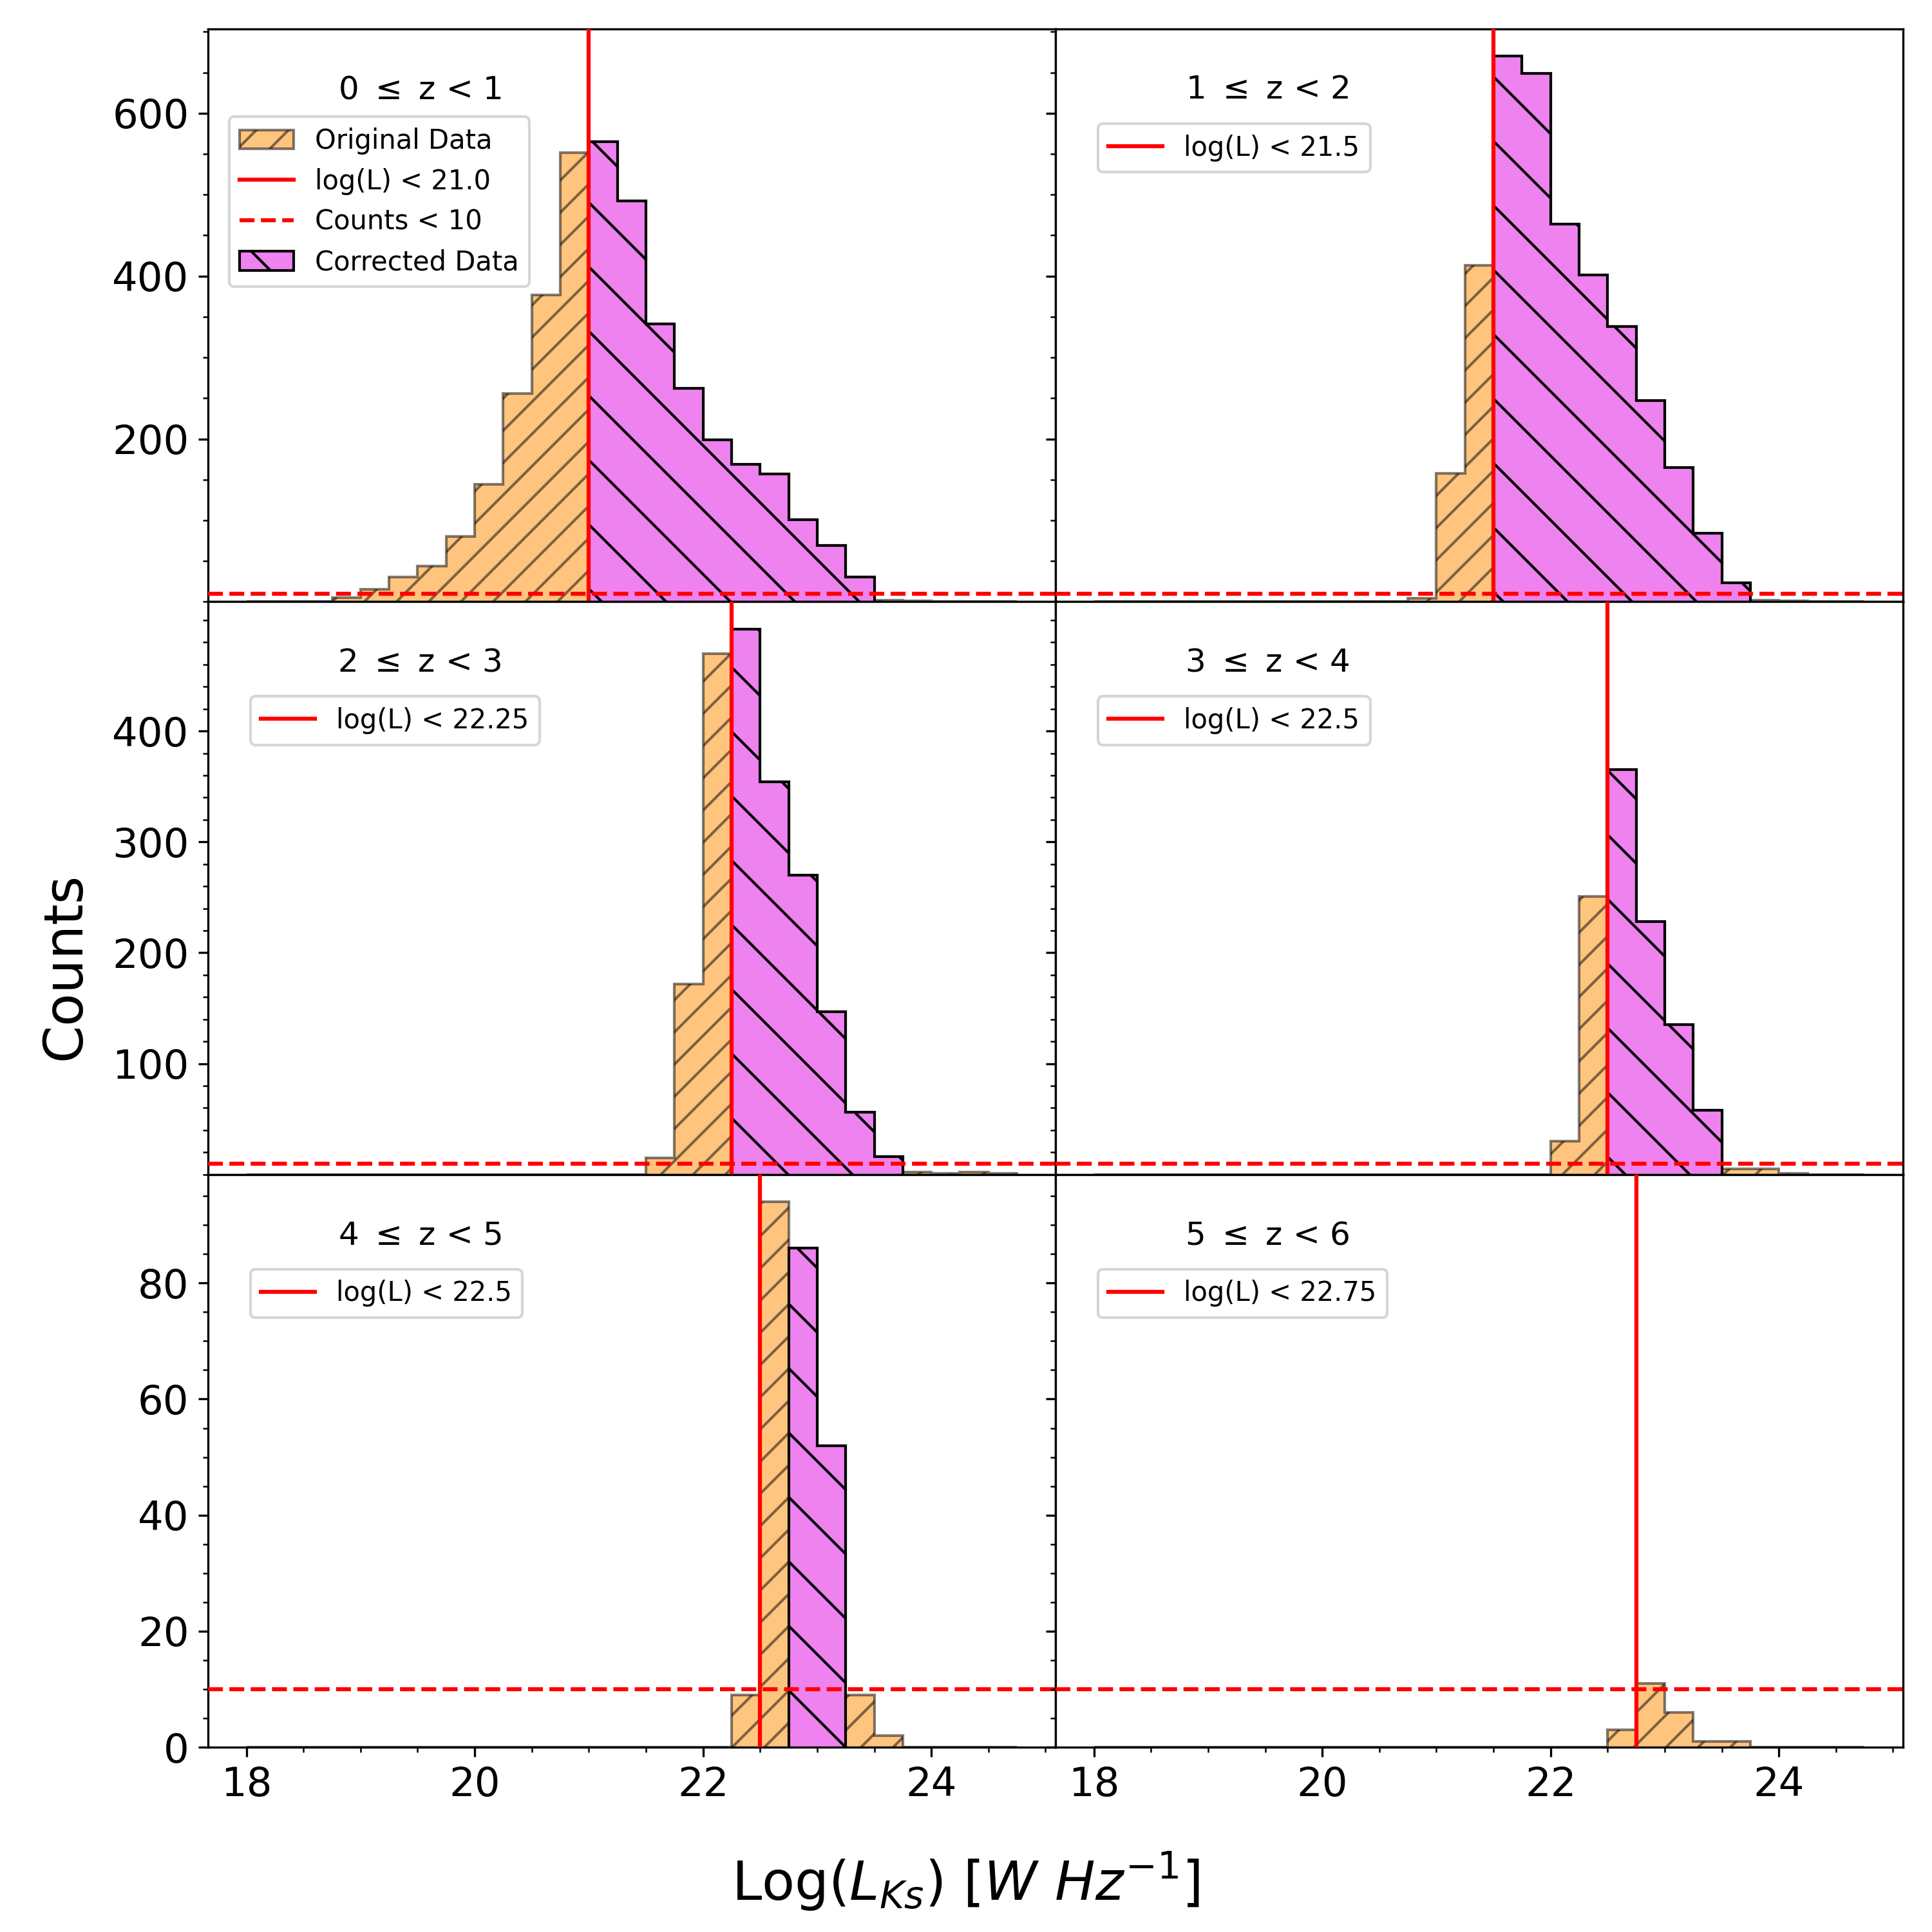
\includegraphics[width=\linewidth]{Figures/Spectral Luminosity Counts.png}
    \caption{Number counts in each redshift and luminosity bin. The red vertical line represents the luminosity completeness limit, varying with each redshift bin. The red dashed horizontal line shows the number completeness limit for each luminosity bin, requiring at least 10 galaxies or else the bin is discarded. Purple bins show the corrected and complete bins, whereas orange bins show incomplete bins.}
    \label{fig: Spectral Luminosity Counts}
\end{figure}

The flux limit in the \texttt{Ks} band is still measured in $AB$ magnitude, which for the CDFS field $F_{lim}=25.9\ [AB]$. This can be converted to $W\ m^{-2}\ Hz^{-1}$ using \cref{EQ: Flux limit from AB}. 

\begin{equation}
    F_{lim,x} [W\ m^{-2}\ Hz^{-1}] = 10^{\frac{F_{lim,x}\ [AB] + 56.1}{-2.5}}
    \label{EQ: Flux limit from AB}
\end{equation}
\myequations{AB Magnitude Flux Limit}

Thus, the flux limit of the \texttt{Ks} band in the \gls{zfourge} CDFS field is $F_{lim}=1.5849\times10^{-33}$ $W\ m^{-2}\ Hz^{-1}$. By calculating the spectral luminosity for every object using \cref{EQ: Luminosity Distance}, the maximum possible distance of each object can now be calculated by rearranging \cref{EQ: Luminosity Distance} and substituting the new flux limit $F_{lim}$ instead of the observed \texttt{Ks} band flux for each object. This effectively calculates the maximum possible distance an object could occur at given we know its intrinsic luminosity, but if its flux were at the survey limit. This is given by \cref{EQ: Maximum Luminosity Distance} below:

\begin{figure}[t!]
    \centering
    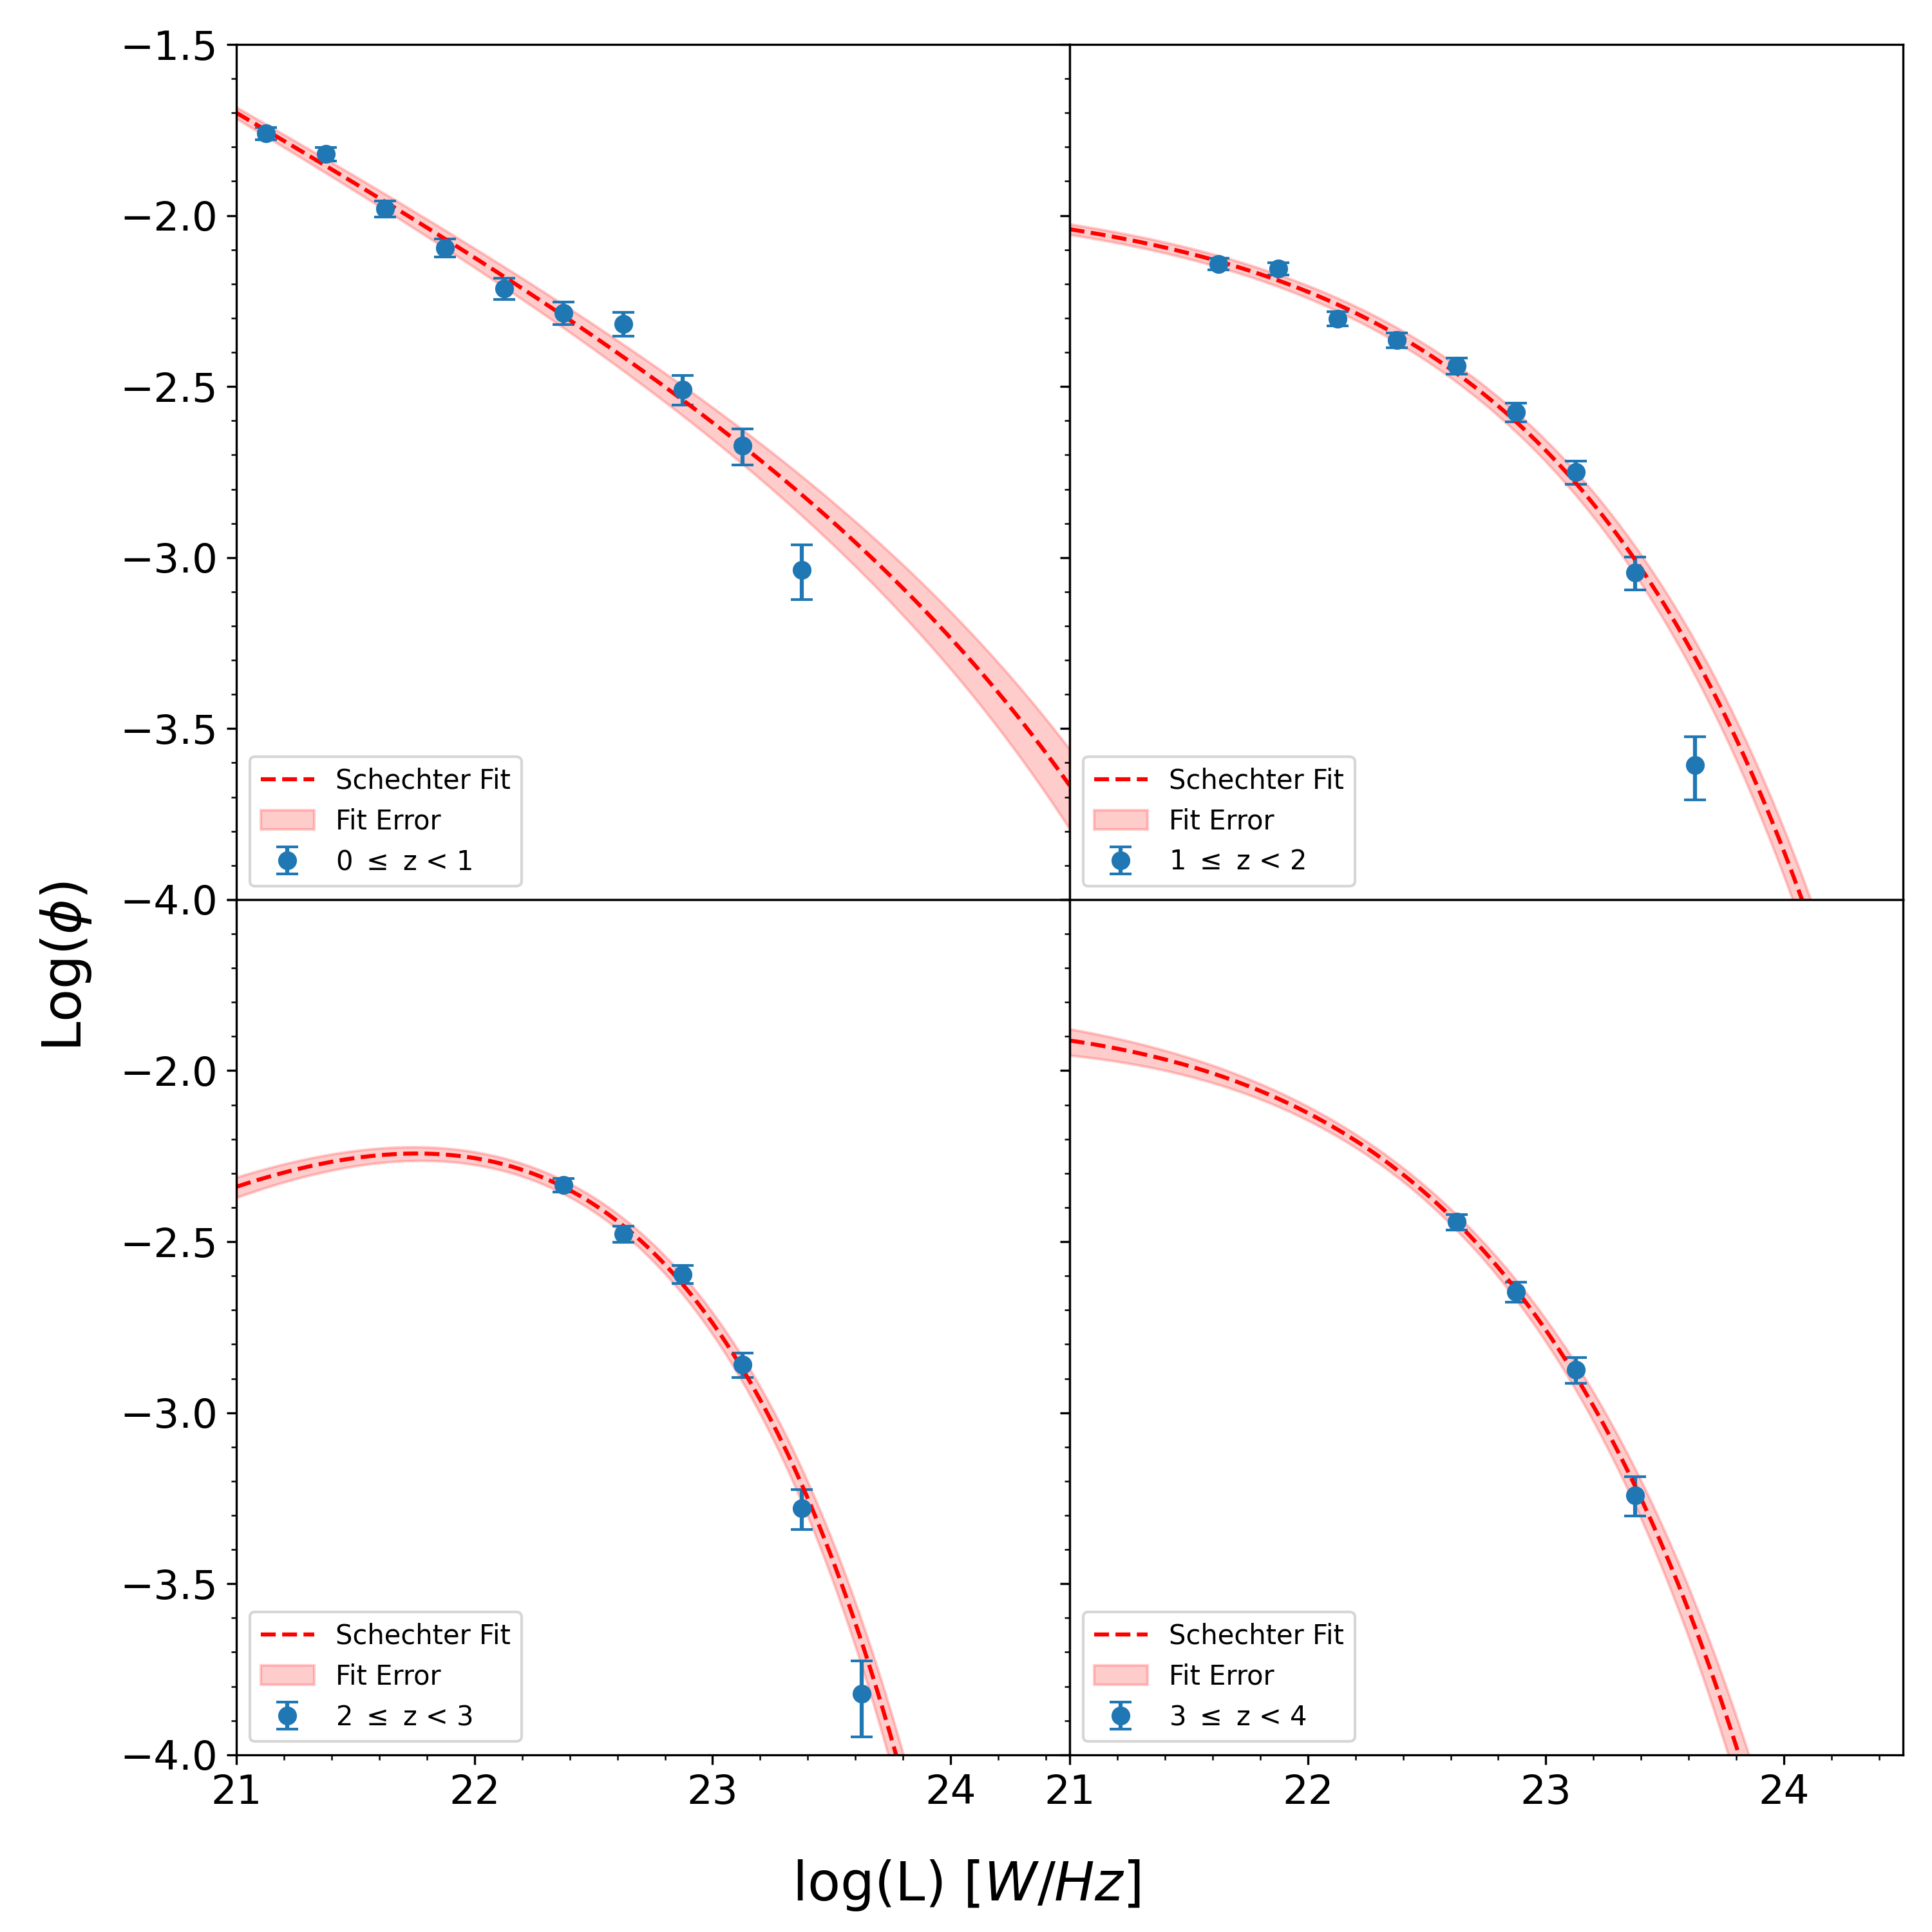
\includegraphics[width=\linewidth]{Figures/Spectral Luminosity Function.png}
    \caption{The Spectral Luminosity Function of the ZFOURGE \texttt{Ks} band. Evolution across four redshift bins is visualised. The redshift bin $4\leq z<5$ had fewer luminosity bins than free parameters so that no LF could be determined. The Schechter function is fit to the luminosity bins in each redshift bin as the red dashed line. The red colour-fill represents the uncertainty of the fit based on the error of each luminosity bin. The luminosity bin errors are simply the $1\sigma$ Poisson errors and do not account for flux errors in \texttt{Ks} or photometric redshift errors.}
    \label{Fig: Spectral Luminosity Function}
\end{figure}

\begin{equation}
    d_{max} = \sqrt{\frac{L}{4 \pi F_{lim}}}
    \label{EQ: Maximum Luminosity Distance}
\end{equation}
\myequations{Maximum Luminosity Distance}

Now that we know the maximum possible distance of each object, we can use \cref{EQ: Vmax} to calculate the maximum observable volume of each source object and thus the \gls{lf}. \Cref{fig: Spectral Luminosity Counts} shows the number count of each luminosity bin in every redshift bin of the \gls{lf}. The luminosity completeness limit (red vertical line) is the peak of the number count distribution. Luminosity bins fainter (to the left) of this limit are excluded (coloured orange) from the \gls{lf} because they are incomplete due to Malmquist sampling bias \citep{malmquist_relations_1922}. The number count completeness limit (red dashed horizontal line) requires a minimum of 10 sources in each luminosity bin. Luminosity bins with less than this limit (below the line) are excluded (coloured orange) from the \gls{lf} because they do not have enough sources to form a well-defined statistical sample. 

The \texttt{Ks} band Spectral \gls{lf} of the \gls{zfourge} CDFS field is presented in \cref{Fig: Spectral Luminosity Function}. The luminosity bins are represented by blue-filled circles with $1\sigma$ Poisson error bars calculated with \cref{EQ: Number Density Error}. To simplify the testing process, we do not include sources of error from photometric redshifts or flux error in the \texttt{Ks} band. The results appear similar to the magnitude luminosity function presented in \cref{fig: Magnitude Function}: the number density of galaxies at low redshift decreases with increasing Ks luminosity and redshift. When the full total IR \gls{lf} are calculated, the errors will be added in quadrature, which is expected to increase the errors. The Schechter function (\cref{EQ: Shechter Function}) is used to fit each redshift bin as the red dashed line and colour filled between the upper and lower uncertainty. The evolution of the \gls{lf} across redshift and luminosity can be used to infer properties about the class of objects studied across the universe's history.